\documentclass[10.5pt]{article}
\usepackage{etex}
\usepackage{amsfonts, amsmath, amssymb}
\usepackage{multirow, multicol}
\usepackage{epsfig, subfigure, subfloat, graphicx}
\usepackage{anysize, indentfirst, setspace}
\usepackage{verbatim, rotating, paralist}
\usepackage{caption, hanging}
\usepackage{pstricks, sgamevar, egameps}
\usepackage{lscape}
\usepackage{tikz}
\usepackage{hyperref}
\usetikzlibrary{shapes,arrows,backgrounds,decorations.pathmorphing,decorations.pathreplacing,calc,fadings}
% These are the key packages.  There is also sgame instead of sgamevar, but it doesn't work with beamer or other macros.
% The dcolumn package interferes with these, so you need to remove it from your preamble.


\title{Drawing Games and Diagrams in \LaTeX \footnote{This handout borrows heavily from the department's 2010 \LaTeX~handout authored by Dave Ohls and 2013 materials from Richard Loeza.}}
\author{Sarah Bouchat}
\date{\today}

\begin{document}


\maketitle

This guide emphasizes a series of ways to draw game matrices and decision trees---both of which will be useful for 835 and 836---as well as providing some basic building blocks for drawing using \LaTeX. This should be considered a very rudimentary introductory guide---there are many more things to learn about drawing and figures in \LaTeX that are omitted here.\\


\section{Strategic Form Games}

Writing strategic form games using the \verb+sgamevar+ package creates diagrams that looks a lot like normal tabular environments, but it has the advantage of automatically tailoring the dimensions and labels to the alignment you want, rather than forcing you to do it by hand. There are a couple of things that distinguish it from a typical table environment:

\begin{compactitem}
\item Use the ``figure'' float instead of the ``table'' float.
\item The \verb+\>+ replaces \verb+&+ as the divider between cells. Note that in the \verb+sgame+ package, you use \verb+&+ still. 
\item The initial operators are different: rather than \verb+\begin{tabular}{l|cc}...\end{tabular}+ it is: \\ \verb+\begin{game}{rows}{columns}[player 1 label][player 2 label][figure label]...\end{game}+ \\
\end{compactitem}

\begin{figure}[h!]
\begin{center}
\begin{footnotesize}
\begin{game}{2}{3}[1][2][]
        \> Left \> Center \> Right   \\
Top      \> 3,2  \> 4,4    \> 2,1   \\
Bottom    \> 1,1  \> 5,7    \> 4, 3 \\
\end{game}
\end{footnotesize}
\end{center}
\end{figure}

Most stylistic commands also work inside games. Using circles to indicate best responses is problematic because the circles tend to cut off some of the numbers. You can also use highlighting.

\begin{figure}[h!]
\begin{footnotesize}
 \begin{center}
\begin{game}{5}{5}[\textbf{1}][\textbf{2}][Ammunition]
       \> Rock    \> Paper   \> Scissors \> Flamethrower \> Water Canon  \\
Rock \> \underline{1,1}  \>  0,2  \> 2,0 \> 2,0 \> 0,2 \\
 Paper \> 2,0    \> \underline{1,1}  \> 0,2 \> 0,2 \> 2,0 \\
 Scissors \> 0,2 \> 2,0 \> \underline{1,1} \> 2,0 \> 0,2 \\
Flamethrower \> 0,2  \> 2,0 \> 0,2 \> \underline{1,1} \> 2,0 \\
 Water Canon \> 2,0 \> 0,2 \> 2,0 \> 0,2 \> \textcircled{1},\textcircled{1} \\
\end{game}
\end{center}
\end{footnotesize}
\end{figure}

\sgcolsep=0.5pt
\renewcommand{\gamestretch}{1.5}
\def\highlight#1{\colorbox{lightgray}{#1}}
\fboxsep=5pt
\begin{figure}[htb]\hspace*{\fill}%
\begin{center}
\begin{game}{3}{3}[{\em Bob}     ][{\em Jim}][]
        \> A \> B \> C   \\
X \>8,6\> 6,8 \> 0,0   \\
Y \> 6,8  \> 8,6 \> 0,0 \\
Z \> 0,0 \> 0,0 \>\highlight{5,5}\\
\end{game} 
\end{center} 
\end{figure}
 

\section{Extensive Form Games}
Previous versions of this workshop used the \verb+egamesps+ package to create extensive form games. That package makes creating extensive games simpler, but it is very prone to errors and much less flexible than using the tikz approach. Be aware that using egamesps may require you to use a different compilation engine for your \LaTeX document (e.g., XeTeX).

\begin{figure}[htb]
\hspace*{\fill}
\begin{egame}(600,280)
\putbranch(300,240)(2,1){200}
\iib{1}{$C_a$}{$D_a$}
\putbranch(100,140)(1,1){100}
\egalhshift=20
\iib{$2_a$}{$C$}{$D$}[$2,2$][$0,3$]
\putbranch(500,140)(1,1){100}
\egalhshift=20
\iib{$2_b$}{$C$}{$D$}[$3,0$][$1,1$]
\end{egame}
\hspace*{\fill}
\caption[]{Sequential PD}
\end{figure}

Instead of dealing with these issues, you can create extensive form games using the \verb+tikzpicture+ environment, from the tikz package. The tikz package is designed for drawing in general, and is very flexible. The package can accommodate nearly any shape or arrangement you desire. The basic syntax of the coding language involves drawing a series of objects (lines, geometric shapes, text), specifying their location on a coordinate scale, and specifying the properties you want them to have (size, style, color, shading, special features). 


\begin{center}
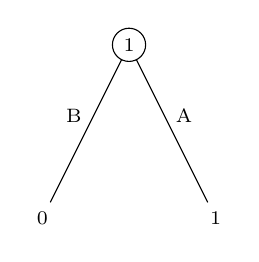
\begin{tikzpicture}[scale=1]
\draw(0,2) -- (1,0);
\draw(0,2) -- (-1,0);
\draw (.7,1.1) node{\scriptsize{A}};
\draw (-.7,1.1) node{\scriptsize{B}};
\draw(1.1,-.2) node {\scriptsize{1}};
\draw(-1.1,-.2) node {\scriptsize{0}};
\filldraw[fill=white](0,2) circle (6pt) node{\scriptsize{1}};
\end{tikzpicture}
\end{center}

What the commands are doing: \\

\begin{compactitem}
\item \verb+[scale=1]+Scales the figure with the dimensions given (in centimeters).  Increase (or decrease) the scale to expand (or shrink) the figure.
\item \verb+\draw (0,2) -- (1,0);+: Draws a straight line between coordinate points (0,2) and (1,0).
\item \verb+\draw (.7,1.1) node{\scriptsize{A}};+ Creates a node with the small text A at the coordinates (.7,1.1).
\item \verb+\filldraw[fill=white](0,2) circle (6pt) node{\scriptsize{1}};+ Creates a circle, 6 points in diameter and fills the inside white. It then creates a small 1 in the middle of the circle. Note that this will cover up anything under the filled circle. 
\end{compactitem}
\vspace{.5cm}
With tikz, the order in which objects are rendered is important. A filled circle will go over anything at the same coordinates if it is listed after those things. Note how the above figure looks when the ordering is changed.

\begin{center}
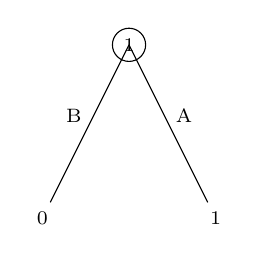
\begin{tikzpicture}[scale=1]
\filldraw[fill=white](0,2) circle (6pt) node{\scriptsize{1}};
\draw(0,2) -- (1,0);
\draw(0,2) -- (-1,0);
\draw (.7,1.1) node{\scriptsize{A}};
\draw (-.7,1.1) node{\scriptsize{B}};
\draw(1.1,-.2) node {\scriptsize{1}};
\draw(-1.1,-.2) node {\scriptsize{0}};
\end{tikzpicture}
\end{center}

Note that every line in a tikzpicture ends in a semicolon. A common error is forgetting to put one in.\\

With these basic tools, you can make games in a variety of shapes.

\begin{center}
\begin{scriptsize}
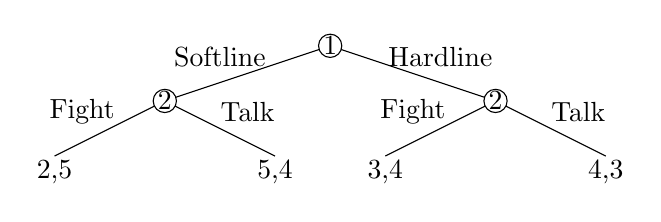
\begin{tikzpicture}[scale=.7]
\draw(7,3) -- (4,2);
\draw(7,3) -- (10,2);
\draw (5,2.8) node{Softline};
\draw (9,2.8) node{Hardline};
\draw(4,2) -- (2,1);
\draw(4,2) -- (6,1);
\draw (2.5,1.8) node{Fight};
\draw (5.5,1.8) node{Talk};
\draw(10,2) -- (8,1);
\draw(10,2) -- (12,1);
\draw (8.5,1.8) node{Fight};
\draw (11.5,1.8) node{Talk};
\filldraw[fill=white](7,3) circle (6pt) node{1};
\filldraw[fill=white](4,2) circle (6pt) node{2};
\filldraw[fill=white](10,2) circle (6pt) node{2};
\draw(2,.7) node {2,5};
\draw(6,.7) node {5,4};
\draw(8,.7) node {3,4};
\draw(12,.7) node {4,3};
\end{tikzpicture}
\end{scriptsize}
\end{center}

\begin{center}
\begin{footnotesize}
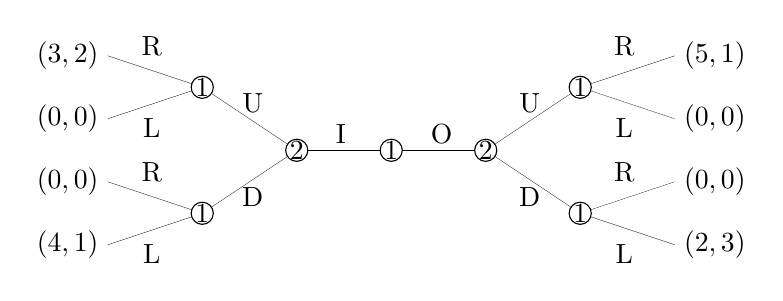
\begin{tikzpicture}[scale=.8]
\draw[ultra thin] (6,0) -- (7.5,1); 
\draw[ultra thin] (6,0) -- (7.5,-1);
\draw[ultra thin] (6,0) -- (4.5,0);
\draw[ultra thin] (3,0) -- (4.5,0);
\draw[ultra thin] (3,0) -- (1.5,1); 
\draw[ultra thin] (3,0) -- (1.5,-1);
\draw (6.7,.75) node{U};
\draw (6.7,-.75) node{D};
\draw (2.3,.75) node{U};
\draw (2.3,-.75) node{D};
\draw (3.7,.25) node{I};
\draw (5.3,.25) node{O};
\filldraw[fill=white] (6,0) circle (5pt) node {2};
\filldraw[fill=white] (3,0) circle (5pt) node {2};
\filldraw[fill=white] (4.5,0) circle (5pt) node {1};
\draw[ultra thin] (7.5,-1) -- (9,-.5) node[right]{$(0,0)$};
\draw[ultra thin] (7.5,-1) -- (9,-1.5) node[right]{$(2,3)$};
\draw (8.2,-.35) node{R};
\draw (8.2,-1.65) node{L};
\draw (8.2,.35) node{L};
\draw (8.2,1.65) node{R};
\filldraw[fill=white] (7.5,-1) circle (5pt) node {1};
\draw[ultra thin] (7.5,1) -- (9,.5) node[right]{$(0,0)$};
\draw[ultra thin] (7.5,1) -- (9,1.5) node[right]{$(5,1)$};
\filldraw[fill=white] (7.5,1) circle (5pt) node {1};
\draw[ultra thin] (1.5,1) -- (0,.5) node[left]{$(0,0)$};
\draw[ultra thin] (1.5,1) -- (0,1.5) node[left]{$(3,2)$};
\draw[ultra thin] (1.5,-1) -- (0,-.5) node[left]{$(0,0)$};
\draw[ultra thin] (1.5,-1) -- (0,-1.5) node[left]{$(4,1)$};
\draw (.7,-.35) node{R};
\draw (.7,-1.65) node{L};
\draw (.7,.35) node{L};
\draw (.7,1.65) node{R};
\filldraw[fill=white] (1.5,1) circle (5pt) node {1};
\filldraw[fill=white] (1.5,-1) circle (5pt) node {1};
\end{tikzpicture}
\end{footnotesize}
\end{center}




\end{document}
